\documentclass[AMA,STIX1COL,]{WileyNJD-v2}


% For Pandoc highlighting needs

% Pandoc citation processing

\usepackage{tikz}
\usepackage{pgfplots}
\usepackage{pdflscape}
\usepackage{color}
\usepackage{soul}
\usepackage{multirow}
\usepackage{multicol}
\usepackage{colortbl}
\usepackage{hhline}
\usepackage{longtable}
\usepackage{array}
\usepackage{hyperref}

\articletype{Research article}

\received{2021-01-01}

\revised{2021-02-01}

\accepted{2021-03-01}

\raggedbottom

\providecommand{\tightlist}{%
  \setlength{\itemsep}{0pt}\setlength{\parskip}{0pt}}

\begin{document}

\title{Spike-and-Slab LASSO Generalized Additive Models and Scalable
Algorithms for High-Dimensional Data Analysis}

\author[a]{Boyi Guo*}
\author[b]{Byron C. Jaeger}
\author[a]{AKM Fazlur Rahman}
\author[a]{D. Leann Long}
\author[a]{Nengjun Yi*}

\authormark{Guo et al.}

\address[a]{Department of Biostatistics, University of Alabama at
Birmingham, Birmingham, USA}
\address[b]{Department of Biostatistics and Data Science, Wake Forest
School of Medicine, Winston-Salem, USA}

\corres{Boyi Guo and Nengjun Yi, Department of Biostatistics, University
of Alabama at Birmingham, Birmingham, USA. \email{boyiguo1@uab.edu},
\email{nyi@uab.edu}}

\presentaddress{This is sample for present address text this is sample
for present address text}

\abstract{There are proposals that extend the classical generalized
additive models (GAMs) to accommodate high-dimensional data (\(p>>n\))
using group sparse regularization. However, the sparse regularization
may induce excess shrinkage when estimating smoothing functions,
damaging predictive performance. Moreover, most of these GAMs consider
an ``all-in-all-out'' approach for functional selection, rendering them
difficult to answer if nonlinear effects are necessary. While some
Bayesian models can address these shortcomings, using Markov chain Monte
Carlo algorithms for model fitting creates a new challenge, scalability.
Hence, we propose Bayesian hierarchical generalized additive models as a
solution: we consider the smoothing penalty for proper shrinkage of
curve interpolation via reparameterization. A novel two-part
spike-and-slab LASSO prior for smoothing functions is developed to
address the sparsity of signals while providing extra flexibility to
select the linear or nonlinear components of smoothing functions. A
scalable and deterministic algorithm, EM-Coordinate Descent, is
implemented in an open-source R package BHAM. Simulation studies and
metabolomics data analyses demonstrate improved predictive and
computational performance against state-of-the-art models. Functional
selection performance suggests trade-offs exist regarding the effect
hierarchy assumption.}

\keywords{Spike-and-Slab Priors; High-Dimensional Data; Generalized
Additive Models; EM-Coordinate Decsent; Scalablility; Predictive
Modeling}

\maketitle

\pgfplotsset{compat=1.18}
\usetikzlibrary{shapes.geometric, arrows, positioning, calc, matrix, backgrounds, fit}
\newcommand{\bs}[1]{\boldsymbol{#1}}
\newcommand{\tp}{*}
\newcommand{\pr}{\text{Pr}}
\newcommand{\repa}{\text{repa}}
\newcommand{\simiid}{\overset{\text{iid}}{\sim}}
\newcommand{\bg}[1]{\textcolor{red}{#1}}

\section{Introduction}
\label{sec:intro}

Much modern biomedical research, e.g., sequencing data analysis and
electronic health record data analysis, require special treatment of
high-dimensionality, commonly known as \(p >> n\) problem. There is
extensive literature on high-dimensional linear models via penalized
models or Bayesian hierarchical models, see Mallick and Yi
\citep{Mallick2013} for review. These models are built upon a
restrictive and unrealistic assumption, linearity. In classical
statistical modeling, many strategies and models are proposed to relax
the linearity assumption with various degrees of complexity. For
example, variable categorization is a simple and common practice in
epidemiology but suffers from power and interpretation issues. More
complex models to address nonlinear effects include random forest and
other so-called ``black box'' models \citep{Breiman2001}. These models
are useful for statistical prediction but do not estimate parameters
relevant to the data generation process that one can draw inferences
from. In addition, how to generalize these \textcolor{red}{"black box"}
models to the high-dimensional setting remains unclear.

\textcolor{red}{For their straightforward interpretation and flexibility, nonparametric regression models serve as great alternatives to the "black-box" models in prediction and variable selection}.
Among those, generalized additive models (GAMs), proposed in the seminal
work of Hastie and Tibshirani \citep{Hastie1987}, grew to be one of the
most popular modeling tools. In a GAM, the response variable, which is
assumed to follow some exponential family distribution, can be modeled
with the summation of smoothing functions. Nevertheless, the classical
GAMs cannot fulfill the increasing analytic demands for high-dimensional
data analysis.

There exist some proposals to generalize the classical GAM to
accommodate high-dimensional applications. The regularized models,
branching out from group regularized linear models, are used to fit GAMs
by accounting for the structure introduced when expanding smoothing
functions. Ravikumar et al. \citep{Ravikumar2009} extended the group
LASSO \citep{Yuan2006} to additive models (AMs); Huang et al.
\citep{Huang2010} further developed adaptive group LASSO for additive
models; Wang et al. \citep{Wang2007} and Xue \citep{Xue2009}
respectively applied group SCAD penalty \citep{Fan2001} to additive
models. Bayesian hierarchical models are also used in the context of
high-dimensional additive models, particularly within the spike-and-slab
literature. Various group spike-and-slab priors \citep{Xu2015, Yang2020}
combining with computationally intensive Markov chain Monte Carlo (MCMC)
algorithms are proposed, where the application on AMs is treated as a
special case. Bai and co-authors\citep{Bai2020} were the first to apply
group spike-and-slab LASSO prior to Gaussian AMs using a fast
optimization algorithm and further generalized the framework to GAMs
\citep{Bai2021}. Focus on addressing the sparsity, these methods can
excessively penalize the bases of a smoothing function and produce
inaccurate predictions, particularly when complex signals are assumed
and large numbers of knots are used. \citep{Scheipl2013} In addition,
these methods adopt an `all-in-all-out' strategy, i.e.~either including
or excluding the variable completely, rendering no space for bi-level
selection. Scheipl et al. \citep{Scheipl2012} proposed a spike-and-slab
structure prior that addresses the bi-level selection. But the model
fitting relies on computationally intensive MCMC algorithms and creates
scalability concerns. Developing a fast, flexible and accurate
generalized additive model framework would be of special interest.

\textcolor{red}{We propose a novel Bayesian hierarchical generalized additive model (BHAM) for outcome prediction in the context of high-dimensional data analysis. Specifically, we incorporate smoothing penalties, derived from the smoothing spline literature \cite{Wood2017}, via reparameterization of smoothing functions to avoid excessive shrinkage on the bases. Smoothing penalties were also previously used in the spike-and-slab GAM \cite{Scheipl2012} and the sparsity-smoothness penalty \cite{Meier2009}. We then impose a new two-part spike-and-slab LASSO prior to address the signal sparsity. In addition, a scalable optimization-based algorithm, EM-Coordinate Descent (EM-CD) algorithm, is developed. While the primary focus of this model is to improve prediction, the proposed model also provides utility in functional selection. Notably, the two-part prior that follows the effect hierarchy principle motivates a bi-level selection, rendering one of three possibilities for each predictor: no effect, only linear effect, or linear and nonlinear effects. The proposed model is implemented in a publicly available R package \texttt{BHAM} via \url{https://github.com/boyiguo1/BHAM}.}

The proposed framework, BHAM, differs from previous spike-and-slab based
GAMs, i.e., the spike-and-slab GAM \citep{Scheipl2012} and the sparse
Bayesian GAM (SB-GAM) \citep{Bai2021}, in three ways. Firstly, the
proposed prior for smoothing functions is a spike-and-slab LASSO type
prior using independent mixture double exponential distribution,
compared to spike-and-slab GAM that uses normal-mixture-of-inverse gamma
prior. Spike-and-slab LASSO priors provide computational convenience
during model fitting by using optimization algorithms instead of
intensive sampling algorithms. They make fitting high-dimensional models
more feasible without sacrificing performance in prediction and variable
selection. Secondly, SB-GAM uses a group spike-and-slab LASSO prior with
an EM-CD algorithm to fit the model. While both methods use the
combination of expectation maximization algorithm and coordinate descent
algorithm, there are subtle differences in the implementation due to the
difference in prior specification. The proposed model sets up
independent priors among basis coefficients after the reparameterization
step, which provides some advantage in computation. Lastly, the proposed
model addresses the incapability of bi-level selection in SB-GAM.

In Section \ref{sec:BHAM}, we establish the Bayesian hierarchical
generalized additive model, introduce the proposed spike-and-slab spline
priors, and describe the fast-fitting EM-CD algorithm. In Section
\ref{sec:sim}, we compare the proposed framework to state-of-the-art
models via Monte Carlo simulation studies. Analyses of two metabolomics
datasets are presented in Section \ref{sec:real_data}. Conclusion and
discussions are given in Section \ref{sec:concl}.

\section{Bayesian Hierarchical Additive Models (BHAM)}
\label{sec:BHAM}

\textcolor{red}{We assume the response variable, $Y$, follows an exponential family distribution with density function $f(y)$, mean $\mu$ and dispersion parameter $\phi$. The mean of the response variable can be modeled as the summation of smoothing functions, $B_j(\cdot), j = 1, \dots, p$, of a given $p$-dimensional vector of predictors $\boldsymbol{x}$, written as 
\begin{equation}\label{eq:gam}
 E(Y|\boldsymbol{x}) = g^{-1}(\beta_0 + \sum\limits^p_{j=1}B_j(x_j)) = g^{-1}(\beta_0 + \sum\limits^p_{j=1} \boldsymbol{\beta}_j^T \boldsymbol{X}_j),
\end{equation}
where $g^{-1}(\cdot)$ is the inverse of a monotonic link function. Given $n$ data points $\{y_i, \boldsymbol{x}_i\}^n_{i=1}$,}
the data distribution is expressed as \begin{equation}
f(\boldsymbol{Y} = \boldsymbol{y}| \boldsymbol{\beta}, \phi) = \prod\limits^n_{i=1}f( Y = y_i|\boldsymbol{\beta}, \phi).\nonumber
\end{equation}

The basis function matrix, i.e.~the design matrix derived from the
smoothing function \(B_j(x_j)\), is denoted \(\boldsymbol{X}_j\) for the
variable \(x_j\). The dimension of the design matrix depends on the
choice of the smoothing function, and is denoted as \(K_j\) for \(x_j\).
\(\boldsymbol{\beta}_j\) denotes the basis function coefficients for the
\(j\)th variable such that
\(B_j(x_j) = \boldsymbol{\beta}_j^T \boldsymbol{X}_j\). With slight
abuse of notation, we denote vectors and matrices in bold fonts
\(\boldsymbol{\beta}, \boldsymbol{X}\) with conformable dimensions,
where scalar and random variables are denoted in unbold fonts
\(\beta, X\). The matrix transposing operation is denoted with a
superscript \(^T\).
\textcolor{red}{To note, the proposed model can include parametric forms of variables in the model, and hence considers general linear models and semiparametric regression models as special cases.}

\subsection{Smoothing Function Reparameterization}

To encourage proper smoothing of each additive function, we adopt the
smoothing penalty from smoothing spline models\citep{Wood2017}. A
smoothing penalty is the quadratic norm of the basis coefficients and
allows different shrinkage on different bases, mathematically
\begin{equation}
  \text{pen}\left[B_j(x)\right] = \lambda_j \int B^{\prime\prime}_j(x)dx = \lambda_j \boldsymbol{\beta}_j^T \boldsymbol{S}_j \boldsymbol{\beta}_j ,\nonumber
\end{equation} where \(\boldsymbol{S}_j\) is a known smoothing penalty
matrix and \(\lambda_j\) denotes a smoothing parameter. A linear
function can be modeled as \(B_j(x_j) = x_j\) with the smoothing penalty
matrix \(\boldsymbol{S}_j = \begin{bmatrix}0\end{bmatrix}\).
\textcolor{red}{Unlike previous regularized methods that either ignore the smoothing penalty completely or restrain the smoothing penalty as a component of sparse penalty which leads to a more restrictive solution, we consider an additional mechanism in pair with the proposed prior (described in Section \ref{sec:method_prior}) to address the smoothness and sparsity in signals such that the locally adaptive nature of the smoothing penalty retains.}

Marra and Wood \citep{Marra2011} proposed a reparameterization procedure
\textcolor{red}{to factor the smoothing penalty into the design matrix of each smoothing function}.
Given that the smoothing penalty matrix \(\boldsymbol{S}_j\) is
symmetric and positive semi-definite for the univariate smoothing
functions, we eigendecompose the penalty matrix
\(\boldsymbol{S} = \boldsymbol{U} \boldsymbol{D} \boldsymbol{U}^T\) ,
where the matrix \(\boldsymbol{D}\) is diagonal with the eigenvalues
arranged in the ascending order. To note, \(\boldsymbol{D}\) can contain
elements of zeros on the diagonal, where the zeros are associated with
the linear space of the smoothing function. For the most popular
smoothing function, cubic splines, the dimension of the linear space is
one. Hereafter, we focus on discussing a uni-dimensional linear space
for simplicity; however, it generalizes easily to the cases where the
linear space is multidimensional. We further write the orthonormal
matrix
\(\boldsymbol{U} \equiv \begin{bmatrix} \boldsymbol{U}^0 : \boldsymbol{U}^{*}\end{bmatrix}\)
containing the eigenvectors as columns in the corresponding order to
\(\boldsymbol{D}\). That is, \(\boldsymbol{U}\) contains the
eigenvectors \(U^0\) with zero eigenvalues for the linear space and
\(\boldsymbol{U}^{*}\) contains the eigenvectors (as columns) for the
non-zero eigenvalues, i.e.~the nonlinear space. We multiply the basis
function matrix \(\boldsymbol{X}\) with the orthonormal matrix
\(\boldsymbol{U}\) for the new design matrix
\({\boldsymbol{X}}^\text{repa}= \boldsymbol{X} \boldsymbol{U} \equiv \begin{bmatrix} X^0 : \boldsymbol{X}^{*} \end{bmatrix}\).
An additional scaling step is imposed on \(\boldsymbol{X}^{*}\) by the
non-zero eigenvalues of \(\boldsymbol{D}\) such that the new basis
function matrix \(\boldsymbol{X}^\ast\) can receive a uniform penalty on
each of its dimensions. With slight abuse of the notation, we drop the
superscript \(^\text{repa}\) and denote
\(\boldsymbol{X}_j \equiv \begin{bmatrix} X_j^0 : \boldsymbol{X}_j^{*} \end{bmatrix}\)
as the basis function matrix for the \(j\)th variable after the
reparameterization. A spline function can be expressed in the matrix
form \[
B_j(x_j) = B_j^0(x_j) + B_j^*(x_j) = \beta_j X^0_j + \boldsymbol{\beta_j^*}^T \boldsymbol{X}_j^*,
\] and the generalized additive model in Equation (\ref{eq:gam}) now is
\begin{equation}\label{eq:gam-repa}
E(Y|\boldsymbol{x}) = g^{-1}(\beta_0 + \sum\limits^p_{j=1} B_j(x_j)) = g^{-1}(\beta_0 + \sum\limits^p_{j=1} \boldsymbol{\beta}_j^T \boldsymbol{X}_j) = g^{-1}\left[\beta_0 + \sum\limits^p_{j=1} (\beta_j X^0_j + {\boldsymbol{\beta}_j^*}^T \boldsymbol{X}_j^*)\right],
\end{equation} where the coefficients
\(\boldsymbol{\beta}_j \equiv \begin{bmatrix} \beta_j : \boldsymbol{\beta}^*_j \end{bmatrix}\)
is an augmentation of the coefficient scalar \(\beta_j\) of linear space
and the coefficient vector \(\boldsymbol{\beta}^*_j\) of nonlinear
space.

To summarize, the reparameterization step provides three benefits.
Firstly, the reparameterization integrates the smoothing penalty matrix
into the design matrix, and encourages models to properly smooth the
nonlinear function when sparsity penalty exists. Secondly, the
eigendecomposition of the smoothing penalty matrix allows the isolation
of the linear space from the nonlinear space, improving the feasibility
of bi-level functional selection. Lastly, the eigendecomposition
facilitates the construction of an orthonormal design matrix, which
makes imposing independent priors on the coefficients possible. This
reduces the computational complexity compared to using a multivariate
priors, and improve the generalizability of the framework to be
compatible with other choices of priors.

\subsection{Two-part Spike-and-Slab LASSO Prior for Smoothing Functions}\label{sec:method_prior}

The family of spike-and-slab regression models is one of the most
commonly used models in high-dimensional data analysis for its utility
in outcome prediction and variable selection.
\textcolor{red}{Among all the spike-and-slab priors, the spike-and-slab LASSO (SSL) prior \cite{Rockova2018b, Rockova2018} is one of the most popular choices because it's highly scalable. The SSL prior is composed of two double exponential distributions with mean 0 and different dispersion parameters, $0 < s_0 < s_1$, mathematically,
\begin{equation} 
\beta | \gamma \sim (1-\gamma)DE(0, s_0) + \gamma DE(0, s_1), 0 < s_0 < s_1.\nonumber
\end{equation}
} The latent binary variable \(\gamma \in \{0,1\}\) indicates whether a
variable \(x\) is included in the model, while the dispersion parameters
\(s_0\) and \(s_1\) control the shrinkage of the coefficient. Given that
both double exponential distributions have a mean of 0 and the latent
indicator \(\gamma\) can only take the value of 0 or 1, the mixture
double exponential distribution can be formulated as one single double
exponential density, \begin{equation} \label{eq:ssl}
\beta | \gamma \sim DE(0, (1-\gamma)s_0 + \gamma s_1), 0 < s_0 < s_1.
\end{equation}
\textcolor{red}{Compared to other priors for high-dimensional data analysis, SSL has the following advantages. First of all, the SSL prior provides a locally adaptive shrinkage when estimating the coefficients. Secondly, the SSL prior encourages a sparse solution, making variable selection straightforward. Thirdly, the SSL prior motivates a scalable algorithm, the EM-CD algorithm, for model fitting, and hence is more feasible for high-dimensional data analysis. We defer to Bai et al. \cite{Bai2021Review} for a detailed discussion.}

We introduce a novel SSL-based prior for smoothing functions in GAMs.
Given the reparameterized design matrix
\(\boldsymbol{X}_j = \begin{bmatrix} X^0_j : \boldsymbol{X}_j^*\end{bmatrix}\)
for the \(j\)th variable, we impose a two-part SSL prior to the
coefficients
\(\boldsymbol{\beta}_j = \begin{bmatrix} \beta_j : \boldsymbol{\beta}_j^*\end{bmatrix}\).
Specifically, the linear space coefficient has an SSL prior and the
nonlinear space coefficients share a group SSL prior,
\begin{align}\label{eq:bham_ssl}
  \beta_{j} | \gamma_{j},s_0,s_1 &\sim DE(0,(1-\gamma_{j}) s_0 + \gamma_{j} s_1) \nonumber \\
  \beta^*_{jk} | \gamma^*_{j},s_0,s_1 &\overset{\text{iid}}{\sim}DE(0,(1-\gamma^*_{j}) s_0 + \gamma^*_{j} s_1), k=1,\dots, K_j
\end{align} where \(\gamma_{j}\in\{0,1\}\) and
\(\gamma^*_{j}\in \{0,1\}\) are two latent indicator variables,
indicating if the model includes the linear effect and the nonlinear
effect of the \(j\)th variable respectively. \(s_0\) and \(s_1\) are
scale parameters, assuming \(0 < s_0 < s_1\) and given. These scale
parameters \(s_0\) and \(s_1\) can be treated as tuning parameters and
optimized via cross-validation, discussed in Section \ref{sec:tune}.

\textcolor{red}{The proposed two-part SSL prior, particularly the group SSL prior of the nonlinear space coefficients, differs from previous group SSL priors \cite{Tang2018, Tang2019}, as the proposed prior follows the effect hierarchy principle. Effect hierarchy refers to the principle that "lower-order effects are more likely to be active than higher-order effects" defined by Chipman\cite{chipman2006prior}. To implement, we consider the shared latent indicator of nonlinear coefficients $\gamma^*_j$}
depends on the value of the linear space latent indicator \(\gamma_j\),
while both latent indicators \(\gamma_j\) and \(\gamma^*_j\) follow a
Bernoulli distribution. While the probability of including the linear
effect is \(\theta_j\), the probability of including the nonlinear
effect is \(\textcolor{red}{\gamma_{j}}\theta_j\). \[
\begin{aligned}
&\gamma_{j} | \theta_j \sim Bin(1, \theta_j) & & 
&\gamma_{j}^*| \textcolor{red}{\gamma_{j}, } \theta_j \sim Bin(1, \textcolor{red}{\gamma_{j}}\theta_j).
\end{aligned}
\]
\textcolor{red}{This is, when the linear effect is not selected, the probability of including the nonlinear effect drops from $\theta_j$ to 0. For computational convenience, we analytically integrate $\gamma_j$ out such that $\gamma_{j}^*| \theta_j \sim Bin(1, \theta_j^2)$ (see the derivation in the Supporting Information).
}

\textcolor{red}{To allow the shrinkage to self-adapt to the sparsity and smoothing pattern of the data, }we
further specify the parameter \(\theta_j\) follows a beta distribution
with given shape parameters \(a\) and \(b\), \[
\theta_j \sim Beta(a, b).
\] The beta distribution is a conjugate prior to the binomial
distribution and hence provides some computation convenience.
\textcolor{red}{Having a prior distribution of $\theta_j$ enables the proposed prior to inherit the selective shrinkage property and self-adaptivity \cite{Bai2021Review} from the classical SSL prior. In other words, when a smoothing function is significant, the coefficients of the smoothing function escape the overall shrinkage and produce a more accurate estimate, particularly in pair with the smoothing penalty implicitly addressed via the reparameterization. Meanwhile, the hyper prior encourages information borrowing across coordinates and hence automatic adjust for different levels of sparsity.}
Hereafter, we refer to the Bayesian hierarchical generalized additive
models with the two-part spike-and-slab LASSO prior as BHAM, and
visually presented in Figure \ref{fig:SSprior}.

\subsection{Scalable EM-Coordinate Descent Algorithm}

\textcolor{red}{Despite the advantage to estimate posterior densities, using MCMC algorithms to fit the proposed model is computationaly prohibited and not feasible for high-dimensional data. Previous research shows the computation performance of MCMC algorithms for spike-and-slab models is bottlenecked for medium-sized data ($p$=25) \cite{George1997}, and substantially slows as $p$ increases modestly in the GAM context \cite{Scheipl2013}. Hence, we consider the optimization algorithms that focus on the maximum a posteriori estimates at the cost of posterior inference. Specifically, we
extend the EM-Coordinate Descent (EM-CD) algorithm to fit BHAMs. Similar to the EMVS algorithm \cite{Rockova2014a} for spike-and-slab models, the EM-CD algorithm is based on the expectation-maximization (EM) algorithm, integrating the Coordinate Descent algorithm in each iterative step to find the posterior mode. The EM-CD algorithm has been well adapted in generalized linear models \cite{Tang2017a}, Cox proportional hazards models \cite{Tang2017}, and their grouped counterparts \cite{Tang2018, Tang2019}. The EM-CD algorithm provides deterministic solutions, which becomes a popular property for reproducible research.}

For BHAMs, we define the parameters of interest as
\(\Theta = \{\boldsymbol{\beta}, \boldsymbol{\theta}, \phi\}\) and
consider the latent binary indicators \(\boldsymbol{\gamma}\) as
nuisance parameters of the model, in other words, the ``missing'' data
in the EM context. Our objective is to find the parameters \(\Theta\)
that maximize the posterior density function, or equivalently the
logarithm of the density function, \[
\begin{aligned}
& \text{argmax}_{\Theta}
\log f(\Theta, \boldsymbol{\gamma}| \textbf{y}, \textbf{X}) \\
&= \log f(\textbf{y}|\boldsymbol{\beta}, \phi) + \sum\limits_{j=1}^p\left[\log f(\beta_j|\gamma_j)+\sum\limits_{k=1}^{K_j} \log f(\beta^{*}_{jk}|\gamma^{*}_{j})\right]\\
& +\sum\limits_{j=1}^{p} \left[ (\gamma_j+\gamma_{j}^{*})\log \theta_j + (2-\gamma_j-\gamma_{j}^{*}) \log (1-\theta_j)\right] +  \sum\limits_{j=1}^{p}\log f(\theta_j),
\end{aligned}
\]\\
where \(f(\textbf{y}|\boldsymbol{\beta}, \phi)\) is the data
distribution and \(f(\theta)\) is the Beta(a, b) density. We choose
non-informative prior for the intercept \(\beta_0\) and the dispersion
parameter \(\phi\); for example, \(f(\beta_0|\tau_0^2)=N(0,\tau_0^2)\)
with \(\tau^2_0\) set to a large value and \(f(\log \phi) \propto 1\).

We use the EM algorithm to find the maximum a posteriori estimate of
\(\Theta\). This is, in the E-step, we calculate the expectation of
posterior density function of
\(\log f(\Theta, \boldsymbol{\gamma}| \textbf{y}, \textbf{X})\) with
respect to the latent indicators \(\boldsymbol{\gamma}\) conditioning on
the parameter values from previous iteration \(\Theta^{(t-1)}\), \[
E_{\boldsymbol{\gamma}|\Theta^{(t-1)}}\log f(\Theta, \boldsymbol{\gamma}| \textbf{y}, \textbf{X}) .
\] Hereafter, we use the shorthand notation
\(E(\cdot)\equiv E_{\boldsymbol{\gamma}|\Theta^{(t-1)}}(\cdot)\). In the
M-step, we find the parameters \(\Theta^{(t)}\) that maximize
\(E\log f(\Theta, \boldsymbol{\gamma}| \textbf{y}, \textbf{X})\).
\textcolor{red}{The parenthesized subscription $^{(t)}$ denotes the parameter estimation at the $t$th iteration.}
The E- and M- steps are iterated until the algorithm converges.

To note here, the log-posterior density of BHAMs (up to additive
constants) can be written as a two-part equation
\[ \log f(\Theta, \boldsymbol{\gamma}| \textbf{y}, \textbf{X}) = Q_1(\boldsymbol{\beta}, \phi) + Q_2 (\boldsymbol{\gamma},\boldsymbol{\theta}),\]
where
\[ Q_1\equiv Q_1(\boldsymbol{\beta}, \phi) = \log f(\textbf{y}|\boldsymbol{\beta}, \phi) + \sum\limits_{j=1}^p\left[\log f(\beta_j|\gamma_j)+\sum\limits_{k=1}^{K_j} \log f(\beta^{*}_{jk}|\gamma^{*}_{jk})\right]\]
and
\[Q_2 \equiv Q_2(\boldsymbol{\gamma},\boldsymbol{\theta}) = \sum\limits_{j=1}^{p} \left[ (\gamma_j+\gamma_{j}^{*})\log \theta_j + (2-\gamma_j-\gamma_{j}^{*}) \log (1-\theta_j)\right] +  \sum\limits_{j=1}^{p}\log f(\theta_j).\]
\(Q_1\) and \(Q_2\) are respectively the log posterior density of the
coefficients \(\boldsymbol{\beta}\) and the log posterior density of the
probability parameters \(\boldsymbol{\theta}\) conditioning on
\(\boldsymbol{\gamma}\). Meanwhile, conditioning on
\(\boldsymbol{\gamma}\), \(Q_1\) and \(Q_2\) are independent and can be
maximized separately for \(\boldsymbol{\beta}, \phi\) and
\(\boldsymbol{\theta}\). With the proposed two-part spike-and-slab LASSO
prior, \(Q_1\) can be treated as penalized likelihood function and
maximization of \(E(Q_1)\) can be solved via the Coordinate Descent
algorithm in each iteration. Coordinate descent is an optimization
algorithm that offers extreme computational advantages, and is famous
for its application in optimizing the \(l_1\) penalized likelihood
function. Maximization of \(E(Q_2)\) can be solved via closed-form
equations following the beta-binomial conjugate relationship.

The density function of the mixture double exponential prior of
coefficient \(\beta\) can be written as \[
f(\beta|\gamma, s_0, s_1) = \frac{1}{2\left[(1-\gamma)s_0 + \gamma s_1\right]}\exp(-\frac{|\beta|}{(1-\gamma)s_0 + \gamma s_1}),
\] and \(E(Q_1)\) can be expressed as a log-likelihood function with
\(l_1\) penalty \begin{equation}\label{eq:Q1_CD}
E(Q_1) = \log f(\textbf{y}|\boldsymbol{\beta}, \phi) - \sum\limits_{j=1}^p\left[E({S_j}^{-1})|\beta_j|+\sum\limits_{k=1}^{K_j}E({S^{*}}^{-1}_{j})|\beta_{jk}|\right],
\end{equation} where \(S_{j} = (1-\gamma_{j}) s_0 + \gamma_{j} s_1\) and
\(S^*_{j} = (1-\gamma^*_{j}) s_0 + \gamma^*_{j} s_1\). To calculate two
unknown quantities \(E({S_j}^{-1})\) and \(E({S^*}^{-1}_j)\), the
posterior probability
\(p_{j} \equiv \text{Pr}(\gamma_{j}=1|\Theta^{(t-1)})\) and
\(p_{j}^*\equiv \text{Pr}(\gamma^*_{j}=1|\Theta^{(t-1)})\) are
necessary, which can be derived via Bayes' theorem. The calculation of
\(p_j^*\) is slightly different from that of \(p_j\), as \(p_j^*\)
depends on the values of the vector \(\boldsymbol{\beta}^*_{j}\) and
\(p_j\) only depends on the scalar \(\beta_j\). The calculation follows
the equations below, \begin{align*}
p_{j} &= \frac{\text{Pr}(\gamma_{j} = 1|\theta_j)f(\beta_{j}|\gamma_{j}=1, s_1) }{\text{Pr}(\gamma_{j} = 1|\theta_j)f(\beta_{j}|\gamma_{j}=1, s_1) + \text{Pr}(\gamma_{j} = 0|\theta_j)f(\beta_{j}|\gamma_{j}=0, s_0)}\\
p^*_{j} &= \frac{\text{Pr}(\gamma^{*}_{j} = 1|\theta_j)\prod\limits_{k=1}^{K_j}f(\beta_{jk}|\gamma^{*}_{j}=1, s_1) }{\text{Pr}(\gamma^{*}_{j} = 1|\theta_j)\prod\limits_{k=1}^{K_j}f(\beta_{jk}|\gamma^{*}_{j}=1, s_1) + \text{Pr}(\gamma^{*}_{j} = 0|\theta_j)\prod\limits_{k=1}^{K_j}f(\beta_{jk}|\gamma^{*}_{j}=0, s_0)}
\end{align*} where \(\text{Pr}(\gamma_{j} = 1|\theta_j) = \theta_j\),
\(\text{Pr}(\gamma_{j} = 0|\theta_j) = 1-\theta_j\),
\(\textcolor{red}{\text{Pr}(\gamma_{j}^*= 1|\theta_j) = \theta_j^2}\),
\(\textcolor{red}{\text{Pr}(\gamma_{j}^*= 0|\theta_j) = 1-\theta^2_j}\),
\(f(\beta|\gamma=1, s_1) = \text{DE}(\beta|0 , s_1)\),
\(f(\beta|\gamma=0, s_0) = \text{DE}(\beta|0 , s_0)\). It is trivial to
show \begin{align*}\label{eq:exp_scale}
&E(\gamma_{j})  = p_{j} & &E(\gamma^{*}_{j}) = p_{j}^{*}\nonumber\\
&E({S}^{-1}_{j}) = \frac{1-p_{j}}{s_0} + \frac{p_{j}}{s_1} & &E({S_{j}^*}^{-1}) = \frac{1-p_{j}^{*}}{s_0} + \frac{p_{j}^{*}}{s_1}.
\end{align*} After replacing the calculated quantities, \(E(Q_1)\) can
be seen as a \(l_1\) penalized likelihood function with the
regularization parameter \(\lambda = E(S^{-1})\), and hence be optimized
via coordinate descent algorithm \citep{Friedman2010}. Independently,
the remaining parameters of interest \(\boldsymbol{\theta}\) can be
updated by maximizing \(E(Q_2)\). As the beta distribution is a
conjugate prior for Bernoulli distribution, \(\boldsymbol{\theta}\) can
be easily updated with a closed-form equation,
\begin{equation}\label{eq:update_theta}
\theta_j = \frac{p_j + p^*_{j} + a - 1 }{a + b}.
\end{equation}

Totally, the proposed EM-CD algorithm is summarized as follows:

\begin{enumerate}
\def\labelenumi{\arabic{enumi})}
\item
  Choose a starting value \(\boldsymbol{\beta}^{(0)}\) and
  \(\boldsymbol{\theta}^{(0)}\) for \(\boldsymbol{\beta}\) and
  \(\boldsymbol{\theta}\). For example, we can initialize
  \(\boldsymbol{\beta}^{(0)} = \boldsymbol{0}\) and
  \(\boldsymbol{\theta}^{(0)} = \boldsymbol{0}.5\)
\item
  Iterate over the E-step and M-step until convergence

  E-step: calculate \(E(\gamma_{j})\), \(E(\gamma^*_{j})\) and
  \(E({S}^{-1}_{j})\), \(E({S^*}^{-1}_{j})\) with estimates of
  \(\Theta^{(t-1)}\) from previous iteration

  M-step:

  \begin{enumerate}
  \def\labelenumii{\alph{enumii})}
  \item
    Update \(\boldsymbol{\beta}^{(t)}\), and the dispersion parameter
    \(\phi^{(t)}\) if exists, using the coordinate descent algorithm
    with the penalized likelihood function in Equation (\ref{eq:Q1_CD})
  \item
    Update \(\boldsymbol{\theta}^{(t)}\) using Equation
    (\ref{eq:update_theta})
  \end{enumerate}
\end{enumerate}

We assess convergence by the criterion:
\(|d^{(t)}-d^{(t-1)}|/(0.1+|d^{(t)}|)<\epsilon\), where
\(d^{(t)} = -2\log f(\textbf{y}| \textbf{X}, \boldsymbol{\beta}^{(t)},\phi^{(t)})\)
is the estimate of deviance at the \(t\)th iteration, and \(\epsilon\)
is a small value (say \(10^{-5}\)).

\subsection{Selecting Optimal Scale Values}
\label{sec:tune}

Our proposed model, BHAM, requires two preset scale parameters (\(s_0\),
\(s_1\)). Hence, we need to find the optimal values for the scale
parameters such that the model reaches its best prediction performance
regarding criteria of preference. This would be achieved by constructing
a two-dimensional grid, consisting of different (\(s_0\), \(s_1\))
pairs. However, previous research suggests the value of slab scale
\(s_1\) has less impact on the final model and is recommended to be set
as a generally large value, e.g.~\(s_1 = 1\), that provides no or weak
shrinkage. \citep{Rockova2018} As a result, we focus on examining
different values of spike scale \(s_0\). Instead of the two-dimensional
grid, we consider a sequence of \(L\) decreasing values
\(\{s_0^l\}: 0 < s_0^1 < s_0^2 < \dots < s_0^L < s_1\). Increasing the
spike scale \(s_0\) tends to include more non-zero coefficients in the
model. A measure of preference calculated with cross-validations (CV),
e.g.~deviance
\textcolor{red}{(defined as model log-likelihood times -2, $-2\log f(\boldsymbol{y}|\boldsymbol{\hat\beta}, \hat\phi)$)},
area under the curve (AUC), mean squared error, can be used to
facilitate the selection of a final model. The procedure is similar to
the LASSO implementation in the widely used R package \texttt{glmnet},
which quickly fits LASSO models over a list of candidate values of
\(\lambda\) and gives a sequence of models for users to choose from.

\section{Simulation Study}
\label{sec:sim}

In this section, we compare the performance of the proposed model to
\textcolor{red}{six alternative models: linear LASSO models,} component
selection and smoothing operator (COSSO) \citep{Zhang2006GAM}, adaptive
COSSO \citep{Storlie2011}, generalized additive models with automatic
smoothing (referred to as \textit{mgcv} hereafter)\citep{Wood2011},
\textcolor{red}{spike-and-slab GAM \cite{Scheipl2012}}, and SB-GAM
\citep{Bai2021}.
\textcolor{red}{We use linear LASSO models as the benchmark, examining the performance when the linearity assumption doesn't hold}.
COSSO is one of the earliest smoothing spline models that consider
sparsity-smoothness penalty. Adaptive COSSO improved upon COSSO by using
adaptive weight for penalties such that the penalty of each functional
component is different for extra flexibility. \textit{mgcv} is one of
the most popular models for nonlinear effect interpolation and
prediction. Nevertheless,
\textcolor{red}{mgcv doesn't support analyses when the number of parameters exceeds the sample size.}
\textcolor{red}{Spike-and-slab GAM employs a spike-and-slab prior for GAM and uses an MCMC algorithm for model fitting.}
SB-GAM is the first spike-and-slab LASSO GAM. We implement linear LASSO
model with R package \texttt{glmnet 4.1-2}, COSSO and adaptive COSSO
with R package \texttt{cosso 2.1-1}, generalized additive models with
automatic smoothing with R package \texttt{mgcv 1.8-31}, spike-and-slab
GAM with R package \texttt{spikeSlabGAM 1.1-15}, and SB-GAM with R
package \texttt{sparseGAM 1.0}. COSSO models and SB-GAM do not provide
flexibility to define smoothing functions, and hence use the default
choices; mgcv, spikeSlabGAM and the proposed model allow customized
smoothing functions and we choose the cubic regression spline. We
control the dimensionality of each smoothing function, 10 bases, for all
different choices of smoothing functions. We use a 5-fold CV with the
default selection criteria to select the final model for linear LASSO
model, COSSO models, SB-GAM and the proposed model. Twenty default
candidates of tuning parameters (\(s_0\) in BHAM, \(\lambda_0\) in
SB-GAM) are examined for SB-GAM and the proposed model that allow user
specification of tuning candidates. All computation was conducted on a
high-performance 64-bit Linux platform with 48 cores of 2.70GHz
eight-core Intel Xeon E5-2680 processors and 24G of RAM per core and R
3.6.2 \citep{R}.

Other related methods for high-dimensional GAMs also exist, notably the
methods of sparse additive models by Ravikumar et al.
\citep{Ravikumar2009}. However, we exclude these methods from the
current simulation study because they demonstrated inferior predictive
performance compared to \textit{mgcv} \citep{Scheipl2013}.

\subsection{Monte Carlo Simulation Study}

We follow the data generating process described in Bai \citep{Bai2021}:
we first generate \(n=500\) training data points with
\(p=4, 10, 50, 100, 200\) predictors respectively, where the predictors
\(\boldsymbol{X}\) are simulated from a multivariate normal distribution
\(\text{MVN}_{n\times p}(0, I_{P})\). We then simulate the outcome \(Y\)
from two distributions, Gaussian and binomial with the identity link and
logit link \(g(x) = \log(\frac{x}{1-x})\) respectively. The mean of each
outcome is derived via the following function \[
\mathbb{E}(Y) = g^{-1}(5 \sin(2\pi x_1) - 4 \cos(2\pi x_2 -0.5) + 6(x_3-0.5) - 5(x_4^2 -0.3))
\] for Gaussian and binomial outcomes. Gaussian outcomes require
specification of dispersion, where we set the dispersion parameter to be
1. In this data generating process, we have \(x_1, x_2, x_3, x_4\) as
the active predictors, while the rest predictors are inactive,
i.e.~\(f_j(x_j) = 0\) for \(j = 4, \dots, p\). Another set of
independent sample of size \(n_{test}=1000\), is created following the
same data generating process, serving as the testing data. We generate
50 independent pairs of training and testing datasets to evaluate the
prediction and variable selection performance of the chosen models,
where training datasets are used to fit the models and testing datasets
are used to calculate metrics of interest.
\textcolor{red}{In addition, we consider the data generating process where all functional forms of the predictors are linear while keeping the rest of simulation parameters the same. This additional set of linear simulations is designed to investigate the flexibility of the proposed model when nonlinear assumptions are not met.}

To evaluate the predictive performance of the models, the statistics,
\(R^2\) for Gaussian model and AUC for binomial model calculated based
on the testing datasets, are averaged across 50 simulations.
\textcolor{red}{To evaluate the variable selection performance of the models, we record the set of variables each method selects and calculate the averaged positive predictive value (precision), true positive rate (recall), and Matthews correlation coefficient (MCC),
\begin{align*}
&\text{precision} = \frac{TP}{PP}\\
&\text{recall} = \frac{TP}{TP+FP}\\
&\text{MCC} = \frac{TP\times TN - FP \times FN}{\sqrt{(TP+FP)(TP+FN)(TN+FP)(TN+FN)}},
\end{align*}
where TP, TN, FP, FN, and PP are true positives, true negatives, false positives, false negatives, and predicted positives respectively. For the methods that don't automatically achieve variable selection, we set the alpha level at 0.05 for \textit{mgcv} that relies on hypothesis testing, and a soft-threshold at 0.5 for spikeSlabGAM given the marginal inclusion probabilities. For the two methods, BHAM and spikeSlabGAM, that are capable of bi-level selection, we record the probability that the linear and nonlinear components of each predictor are selected in the models.}

\subsection{\textcolor{red}{Simulation Results}}
\subsubsection{\textcolor{red}{Prediction Performance}}

\textcolor{red}{Among the set of simulations where the functional forms of the predictors are nonlinear,}
the predictive performances have a consistent pattern across the two
distributions of outcomes. For simplicity, we use Gaussian simulations
to exemplify the improvement of BHAM and defer to Tables \ref{tab:gaus}
and \ref{tab:bin_auc} for detailed statistics.
\textcolor{red}{The proposed model, BHAM, predicts as good as, if not better than, other high dimensional additive models. Specifically, BHAM shows great improvement over COSSO methods, resulting in a median (interquartile range, IRT) 31\% (131\%) and 20\% (129\%) improvement over COSSO and adaptive COSSO in $R^2$ statistics respectively. The improvement over the spikeSlabGAM model is moderate, resulting in a median (IRT) 6\% (10\%) improvement in $R^2$. When comparing to SB-GAM, BHAM performs better (median (IRT) 13\% (8\%) improvement in R2) in lower dimensional cases ($p=4,10$), and equally good or slightly worse (median (IRT) 1\% (9\%) improvement in R2: ) in high-dimensional cases ($p=50,100, 200$). As previously hypothesized, the linear LASSO model predicts less accurate than other flexible models across all scenarios; mgcv performs extremely well in low-dimensional cases ($p = 4, 10$), and deteriorates as the dimensionality increases until not applicable. To note, mgcv fits models but fails to converge within the default number of iterations when the sample size approaches the number of coefficients to estimate ($p=50$), which leads to bad performance.}
Even though SB-GAM has slight prediction advantage over the proposed
model in high-dimensional situations, the BHAM has an extreme
computational advantage over SB-GAM, resulting median (IRT) 64\% (39\%)
reduction in computation time (measured in seconds) for Gaussian
simulations, without sacrificing much of the prediction accuracy (see
Table \ref{tab:time_sim}).

\textcolor{red}{We also examine the prediction performance when the functional form of predictors is linear, see Supporting Information Table S1, and S2. The proposed model, BHAM, has a similar performance as the linear LASSO model regardless of the distribution. This observation demonstrates that BHAM is a flexible model, and has good prediction performance regardless of the underlying functional form of predictors. spikeSlabGAM has a similar prediction performance to BHAM. Surprisingly, SB-GAM doesn't perform well in high-dimensional Gaussian outcome scenarios.}

\textcolor{red}{\subsubsection{Variable Selection Performance}}
\textcolor{red}{Among the set of simulations where the functional forms of the predictors are nonlinear, the proposed model, BHAM, has a consistent performance across different dimensions and distribution settings (See Table \ref{tab:sim_gaus_var_select} for Gaussian outcomes, and Support Information Table S3 for binomial outcomes): being conservative. The symptoms of conservative variable selection are high precision and low recall, where high precision means that among all the selected variables, high percentage of them are true signals; low recall means that the model selected a small subset among all the active predictions. In other words, BHAM tends to select a smaller set of variables that are truly effective to the outcome. We want to note, the variable selection performance of BHAM is plummeted and not optimized when $p=200$. Upon further investigation, we discover it's because the generic sequence of $s_0$ used to tune the model doesn't contain the optimal value. Overall, among all the models examined, SB-GAM has the best performance, both high precision and high recall, and yields a high MCC. The performance of another Bayesian model, spikeSlabGAM deteriorates as the sparsity grows, particularly when ($p>50$), or for binomial outcomes. The variable selection performance for linear simulations matches with prediction performance: BHAM performs great among the Gaussian scenarios, while the performance of SB-GAM deteriorates.}

\textcolor{red}{Among the high-dimensional methods of comparison, there are two methods that are capable to achieve bi-level selection, the proposed BHAM and spikeSlabGAM. Among the linear simulations, both methods can accurately select the linear components and have a drastically lowered probability, close to 0, to include the nonlinear component, as anticipated. Specifically, spikeSlabGAM have a smaller probability to include the nonlinear component in the model than BHAM. However, this advantage of spikeSlabGAM over BHAM is less obvious among the nonlinear simulations: spikeSlabGAM performs better than BHAM when selecting components of the functional forms that include only linear or nonlinear component, e.g. functional forms for $x_3$ and $x_4$. However, spikeSlabGAM inclines to ignore variables that have more complex function forms, e.g. function forms for $x_1$ and $x_2$. In contrast, BHAM is more likely to include them in the model. This trade-off is determined by the assumption implicitly reflected via the prior hierarchy. We defer an in-depth discussion to Section \ref{sec:concl}.}

\section{Metabolomics Data Analysis}
\label{sec:real_data}

In this section, we apply the proposed model BHAM to analyze two
published metabolomics datasets where the outcomes are binary and
continuous respectively. We demonstrate the improved prediction
performance compared to the other Bayesian hierarchical additive model,
SB-GAM \citep{Bai2021}, while being computationally efficient (see Table
\ref{tab:time_real_data}).
\textcolor{red}{BHAM requires roughly 10\% of the computation time of SB-GAM to fit models.}

\subsection{Emory Cardiovascular Biobank}
\label{sec:ECB}

We use the proposed model BHAM to analyze a metabolic dataset from a
recently published research \citep{Mehta2020} studying plasma
metabolomic profile on the three-year all-cause mortality among patients
undergoing cardiac catheterization. The dataset is publicly available
via \textit{Dryad} \citep{Mehta2020_data}. It contains in total of 776
subjects from two cohorts. As there is a large number of non-overlapping
features among the two cohorts, we use the cohort with a larger sample
size (N=454). There are initially 6796 features in the dataset, which is
too large to be practically meaningful to analyze. Hence, we choose the
top 200 features \textcolor{red}{with the largest variance}. We use
5-knot spline additive models for binary outcome using two different
models, the proposed BHAM and the SB-GAM. 10-Fold CV are used to choose
the optimal tuning parameters of each framework with respect to the
default selection criterion implemented in the software. Out-of-bag
samples are used for prediction performance evaluation, where deviance,
AUC, Brier score, defined as
\(\frac{1}{n}\sum\limits^{n}_{i=1}(y_i - \hat y_i)^2\), and
misclassification error, defined as
\(\frac{1}{n}\sum\limits^{n}_{i=1}I(|y_i - \hat y_i|>0.5)\) are
calculated. BHAM obtains superior AUC, Brier score, and
misclassification error in the out-of-bag samples compared to SB-GAM
(see Table \ref{tab:ECB_res}).
\textcolor{red}{We plot the 33 features included in the final BHAM model in Figure \ref{fig:ECB_fig}.}

\subsection{Weight Loss Maintenance Cohort}

We use the proposed model BHAM to analyze metabolomics data from a
recently published study \citep{Bihlmeyer2021} on the association
between metabolic biomarkers and weight loss, where the dataset is
publicly available \citep{Bihlmeyer2021_data}. In this analysis, we
primarily focus on the analysis of one of the three studies included,
weight loss maintenance cohort \citep{Svetkey2008}, due to the
drastically different intervention effects. In the dataset, 765
metabolites in baseline plasma collected were profiled using liquid
chromatography mass spectrometry. Quality control and natural log
transformation \textcolor{red}{were previously} performed and documented
\textcolor{red}{by the study publishing team \cite{Bihlmeyer2021}}. The
outcome of interest is standardized percent change in insulin
resistance, and hence modeled using a Gaussian model. After removing
missing datapoints and addressing outliers in the data, there are
\(p\)=237 features remaining in the analysis. 5-Knot spline additive
models for the Gaussian outcome are constructed using two different
models, the proposed BHAM and the SB-GAM. 10-Fold CV are used to choose
the optimal tuning parameters of each framework with respect to the
default selection criterion implemented in the software. Out-of-bag
samples are used for prediction performance evaluation, where deviance,
\(R^2\), mean squared error (MSE) defined as
\(\frac{1}{n}\sum\limits^{n}_{i=1}(y_i - \hat y_i)^2\), and mean
absolute error (MAE) defined as
\(\frac{1}{n}\sum\limits^{n}_{i=1}|y_i - \hat y_i|\) are calculated.
BHAM obtains superior \(R^2\), MSE, and MAE in the out-of-bag samples
compared to SB-GAM (see Table \ref{tab:WLM_res}).

\section{Discussion}
\label{sec:concl}

\textcolor{red}{In the paper, we described a novel high-dimensional generalized additive model with Bayesian hierarchical prior for the purpose of predictive modeing. In particular, we introduce a two-part spike-and-slab LASSO prior for reparameterized smoothing functions and derive a scalable EM-CD algorithm for model fitting. The proposed model provides a new angle to address the excess shrinkage of smoothing functions that is commonly vulnerable to previous regularized high-dimensional GAMs, and hence improves the predictive performance. Th EM-CD algorithm, extended from previous spike-and-slab LASSO models, provides a computationally efficient alternative to the computational prohibitive MCMC algorithms, enhancing the scalability of spike-and-slab models. In addition, the two-part prior motivates the bi-level selection of predictors, selection of linear and nonlinear components. In the simulation study and real-data analyses, the proposed model demonstrates improvement in prediction and computational advantage when compared to the state-of-the-art models. When serving the purpose of variable selection, trade-offs exist among methods of comparison.}
We implement the proposed model in an open-source R package
\texttt{BHAM}, deposited at \url{https://github.com/boyiguo1/BHAM}. To
maximize the flexibility of smoothing function specification, we deploy
the same programming grammar as in the state-of-the-art package
\texttt{mgcv}, in contrast to previous tools where smoothing functions
are limited to the default ones. Ancillary functions are provided for
model specification in high-dimensional settings, curve plotting and
functional selection.

The proposed model shares many commonalities with the SB-GAM
\citep{Bai2021}, which is independently developed around the same time
as the proposed work. Both frameworks emphasize computational efficiency
by deploying group spike-and-slab LASSO type priors and
optimization-based scalable algorithms. Bai provides the theoretical
proof for the consistency of variable selection using group
spike-and-slab LASSO prior.
\textcolor{red}{The proposed model focuses on improving prediction performance for high-dimensional GAM, with the capability of bi-level selection. Moreover, the proposed model can easily generalize to other families of priors and smoothing functions if desired. Not focused in this manuscript, the generalization is described in the Supporting Information.}

\textcolor{red}{During designing and analyzing the simulation study, we made couple of interesting observations. First of all, variable selection is a delicate topic in the context of predictive modeling. When prediction performance is used to tune a model, the model could possibly include noise variables in models, for example LASSO and LASSO-based models. \cite{Wu2019} Moreover, bi-level selection is a more complex problem than variable selection. The complexity shows on the validity of the effect hierarchy principle. While most functional forms follow that the linear component exists in the nonlinear function, there are functions that don't follow it, e.g. $x^2$. The proposed prior and spikeSlabGAM employ different structures: the proposed prior imposes effect hierarchy while spikeSlabGAM treats the selection of linear and nonlinear components independent. The different prior setups lead to trade-offs for the purpose of bi-level selection. We recommend to use more judgment in bi-level selection, either relying on heuristic knowledge to choose appropriate prior or exploring multiple models when heuristic knowledge doesn't exist. Secondly, we find the performance of the proposed model is more sensitive to the granularity of $s_0$ sequence in the high-dimensional settings than in the lower dimension settings. Even though the current default sequence of $s_0$ can result in reasonable performance shown in the simulation studies, we recommend fine-tuning the model with a granular sequence of $s_0$ for performance improvement.}

Our future efforts are direct to
\textcolor{red}{uncertainty inference of the proposed model}, survival
analysis and integrative analysis.
\textcolor{red}{Using EM-CD algorithm to fit the proposed BHAM is incapable of conducting uncertainty inference. We derive the EM-Iterative Weighted Least Square algorithm (EM-IWLS, see the Supporting Information) as an alternative. Instead of the Coordinate Descent algorithm, we use the Iterative Weighted Least Square algorithm in the EM procedure. The EM-IWLS algorithm is previously used to fit Bayesian high-dimensional generalized linear models \cite{Yi2012}, and deliver estimates of the coefficient variance-covariance matrix. Due to the space limit, technical details will be explained in a future manuscript.}
While the proposed model addresses a great deal of analytic problems,
analyzing the time-to-event outcome remains unsolved. A naive approach
would be convert a time-to-event outcome to a Poisson outcome following
Whitehead \citep{Whitehead1980}. However, it would be more efficient to
directly fit Cox models via penalized pseudo likelihood function
\citep{Simon2011}. Meanwhile, with the growing understanding of
biological structure within -omics field, it is appealing to integrate
external biology information in the modeling process. The main
motivation for integrative models is that biologically informed grouping
of weak effects increases the power of detecting true associations
between features and the outcome \citep{Peterson2016}, and stabilizes
the analysis results for reproducibility purposes. Such integration can
be achieved by setting up a structural hyperprior on the inclusion
indicator of the smoothing function null space
\(\boldsymbol{\gamma}^0\). A similar strategy has been used in Ferrari
and Dunson \citep{Ferrari2020}.

\clearpage

\bibliography{bibfile.bib}

\clearpage

\begin{figure}
\centering
\begin{tikzpicture} [
staticCompo/.style = {rectangle, minimum width=1cm, minimum height=1cm,text centered, draw=black, fill=blue!30},
outCome/.style={ellipse, minimum width=3cm, minimum height=1cm,text centered, draw=black, fill=blue!30},
mymatrix/.style={matrix of nodes, nodes=outCome, row sep=1em},
PriorBoarder/.style={rectangle, minimum width=5cm, minimum height=10cm, text centered, fill=lightgray!30},
background/.style={rectangle, fill=gray!10,inner sep=0.2cm, rounded corners=5mm}
]

\matrix (linearPrior) [matrix of nodes, column sep = 0mm, row sep = 0.7cm] {
  \node (linearGamma) [outCome] { $\gamma_j \sim Bin(1, \theta_j) $ };\\
  \node (linearBeta) [outCome] { $\beta_j \sim DE(0,(1-\gamma_{j}) s_0 + \gamma_{j} s_1)$};\\
};
\matrix (penPrior) [right = 2cm of linearPrior, matrix of nodes, column sep = 0mm, row sep = 0.7cm] {
  \node (penGamma) [outCome] { $\gamma_{j}^*\sim Bin(1, \textcolor{red}{\gamma_{j}}\theta_j)$ };\\
  \node (penBeta) [outCome] { $\beta_{jk}^*\sim  DE(0,(1-\gamma^*_{j}) s_0 + \gamma^*_{j} s_1)$};\\
};


\node (s) [staticCompo]  at ($(linearBeta)!0.5!(penBeta)$)  {($s_0, s_1$)};
\node (Beta) [staticCompo, below = 1cm of s] {$\boldsymbol{\beta }= (\beta_1, \boldsymbol{\beta}^*_1, \dots,\beta_j, \boldsymbol{\beta}^*_j , \dots,\beta_p, \boldsymbol{\beta}^*_p) $};
\node (Theta)[outCome, above = 2cm of s] {$\theta_{j} \sim Beta(a, b)$};
\node (ab)[staticCompo, above = 0.5cm of Theta] {$(a, b)$};
\node (Y) [outCome, below = 1cm of Beta] {$y_i \sim Expo. Fam. (g^{-1}(\boldsymbol{\beta}^T \boldsymbol{X}_i), \phi)$};

\draw[->] (Theta) -- (linearGamma);
\draw[->] (Theta) -- (penGamma);
\draw[->] (linearGamma) -- (linearBeta) ;
\draw[->] (penGamma) -- (penBeta);
\draw[->, draw = red] (linearGamma) -- (penGamma);
\draw[->] (ab) -- (Theta);
\draw[->] (s) -- (linearBeta) ;
\draw[->] (s) -- (penBeta);
\draw[->] (linearBeta) -- (Beta);
\draw[->] (penBeta) -- (Beta);
\draw[->] (Beta) --  (Y);


\begin{pgfonlayer}{background}
  \node [background,
   fit=(linearGamma) (linearBeta),
   label=above:Linear Space:] {};
  \node [background,
    fit=(penGamma) (penBeta),
    label=above:Nonlinear Space:] {};
\end{pgfonlayer}

\end{tikzpicture}

\caption{Directed acyclic graph of the proposed Bayesian hierarchical additive model with parameter expansion. Elliposes are stochastic nodes, rectangles and are deterministic nodes. }
\label{fig:SSprior}
\end{figure}

\clearpage
\begin{table}[ht]
\centering
\begin{tabular}{cccccccc}
  \hline
P & mgcv & LASSO & COSSO & Adaptive COSSO & BHAM & SB-GAM & spikeSlabGAM \\ 
  \hline
  4 & 0.90 (0.01) & 0.33 (0.01) & 0.71 (0.13) & 0.72 (0.11) & 0.90 (0.01) & 0.79 (0.04) & 0.80 (0.00) \\ 
   10 & 0.90 (0.01) & 0.33 (0.01) & 0.66 (0.21) & 0.77 (0.02) & 0.89 (0.01) & 0.79 (0.04) & 0.79 (0.00) \\ 
   50 & 0.86 (0.02) & 0.32 (0.01) & 0.46 (0.19) & 0.57 (0.18) & 0.80 (0.02) & 0.78 (0.05) & 0.78 (0.01) \\ 
  100 & - & 0.32 (0.01) & 0.41 (0.23) & 0.48 (0.25) & 0.79 (0.01) & 0.79 (0.05) & 0.77 (0.01) \\ 
  200 & - & 0.32 (0.01) & 0.39 (0.19) & 0.40 (0.17) & 0.79 (0.01) & 0.78 (0.04) & 0.75 (0.01) \\ 
   \hline
\end{tabular}
\caption{The average and standard deviation of the out-of-sample $R^2$ measure for
    Gaussian outcomes over 50 iterations. The models of comparison include the proposed Bayesian
    hierarchical additive model (BHAM), component selection and smoothing operator (COSSO), adaptive
    COSSO, mgcv and sparse Bayesian generalized additive model (SB-GAM). mgcv doesn't provide estimation
    whe number of parameters exceeds sample size i.e. p = 100, 200.} 
\label{tab:gaus}
\end{table}

\clearpage
\begin{table}[ht]
\centering
\begin{tabular}{cccccccc}
  \hline
P & mgcv & LASSO & COSSO & Adaptive COSSO & BHAM & SB-GAM & spikeSlabGAM \\ 
  \hline
  4 & 0.94 (0.01) & 0.83 (0.01) & 0.90 (0.01) & 0.90 (0.01) & 0.92 (0.01) & 0.92 (0.01) & 0.90 (0.00) \\ 
   10 & 0.92 (0.03) & 0.83 (0.00) & 0.86 (0.04) & 0.86 (0.03) & 0.92 (0.01) & 0.92 (0.01) & 0.90 (0.00) \\ 
   50 & 0.76 (0.03) & 0.83 (0.01) & 0.83 (0.02) & 0.84 (0.02) & 0.90 (0.01) & 0.92 (0.01) & 0.89 (0.01) \\ 
  100 & - & 0.83 (0.01) & 0.83 (0.02) & 0.81 (0.09) & 0.90 (0.01) & 0.92 (0.01) & 0.88 (0.01) \\ 
  200 & - & 0.83 (0.01) & 0.81 (0.06) & 0.82 (0.05) & 0.88 (0.02) & 0.92 (0.01) & 0.87 (0.02) \\ 
   \hline
\end{tabular}
\caption{The average and standard deviation of the out-of-sample area under the curve measures
    for binomial outcomes over 50 iterations. The models of comparison include the proposed Bayesian
    hierarchical additive model (BHAM), component selection and smoothing operator (COSSO),
    adaptive COSSO, mgcv and sparse Bayesian generalized additive model (SB-GAM). mgcv doesn't provide
    estimation whe number of parameters exceeds sample size i.e. p = 100, 200.} 
\label{tab:bin_auc}
\end{table}

\clearpage
\begin{sidewaystable}[!h]
\centering
\begin{tabular}{lrllllll}
  \hline
Distribution & P & mgcv & COSSO & Adaptive COSSO & BHAM & SB-GAM & spikeSlabGAM \\ 
  \hline
Binomial &   4 & 0.18 (0.04) & 3.16 (1.39) & 5.51 (4.07) & 2.73 (0.22) & 347.17 (89.43) & 8.41 (0.91) \\ 
  Binomial &  10 & 3.46 (11.06) & 8.30 (1.70) & 10.66 (5.30) & 4.08 (0.29) & 539.05 (135.55) & 20.36 (2.16) \\ 
  Binomial &  50 & 660.31 (141.53) & 103.41 (20.00) & 118.82 (18.45) & 14.22 (0.58) & 1590.09 (142.19) & 236.73 (14.83) \\ 
  Binomial & 100 & - & 662.61 (125.00) & 672.65 (185.09) & 31.61 (2.56) & 2720.53 (250.43) & 967.97 (186.85) \\ 
  Binomial & 200 & - & 5325.66 (995.60) & 4963.93 (1482.11) & 82.17 (3.29) & 4788.76 (420.64) & 3371.88 (194.02) \\ 
  Gaussian &   4 & 0.05 (0.01) & 0.75 (0.09) & 0.75 (0.11) & 8.78 (1.57) & 38.82 (2.74) & 1.84 (0.18) \\ 
  Gaussian &  10 & 0.32 (0.39) & 3.42 (0.24) & 3.41 (0.23) & 20.77 (3.95) & 76.12 (5.55) & 5.93 (0.57) \\ 
  Gaussian &  50 & 72.03 (57.99) & 33.98 (2.88) & 34.35 (2.86) & 285.73 (12.53) & 374.76 (23.79) & 65.18 (8.12) \\ 
  Gaussian & 100 & - & 117.79 (3.33) & 119.63 (3.66) & 372.01 (56.92) & 640.44 (21.91) & 194.14 (8.09) \\ 
  Gaussian & 200 & - & 518.86 (40.78) & 524.76 (39.15) & 471.46 (72.23) & 1300.70 (72.74) & 738.52 (62.76) \\ 
   \hline
\end{tabular}
\caption{The average and standard deviation of computation time in seconds,
      including cross-validation and final model fitting, over 50 iterations. The models
      of comparison include the proposed Bayesian hierarchical additive model (BHAM) fitted
      with Iterative Weighted Least Square (BHAM-IWLS) and Coordinate Descent (BHAM-CD)
      algorithms, component selection and smoothing operator (COSSO), adaptive COSSO,
      mgcv and sparse Bayesian generalized additive model (SB-GAM). mgcv doesn't 
      provide estimation whe number of parameters exceeds sample size i.e. p = 100, 200.} 
\label{tab:time_sim}
\end{sidewaystable}

\clearpage
\begin{table}[ht]
\centering
\begin{tabular}{cccccccc}
  \hline
P & Metric & LASSO & COSSO & Adaptive COSSO & BHAM & SB-GAM & spikeSlabGAM \\ 
  \hline
  4 & Precision & 1.00 & 1.00 & 1.00 & 1.00 & 1.00 & 1.00 \\ 
   10 & Precision & 0.76 & 0.84 & 0.93 & 0.62 & 0.86 & 1.00 \\ 
   50 & Precision & 0.48 & 0.70 & 0.69 & 0.88 & 0.75 & 1.00 \\ 
  100 & Precision & 0.43 & 0.61 & 0.59 & 0.99 & 0.79 & 0.99 \\ 
  200 & Precision & 0.36 & 0.61 & 0.47 & 0.28 & 0.75 & 0.99 \\ 
    4 & Recall & 0.53 & 0.49 & 0.53 & 0.88 & 0.99 & 0.51 \\ 
   10 & Recall & 0.40 & 0.52 & 0.52 & 0.83 & 1.00 & 0.50 \\ 
   50 & Recall & 0.35 & 0.40 & 0.48 & 0.37 & 1.00 & 0.50 \\ 
  100 & Recall & 0.33 & 0.36 & 0.40 & 0.30 & 0.99 & 0.50 \\ 
  200 & Recall & 0.32 & 0.33 & 0.35 & 0.52 & 1.00 & 0.50 \\ 
   10 & MCC & 0.32 & 0.49 & 0.57 & 0.46 & 0.86 & 0.61 \\ 
   50 & MCC & 0.31 & 0.47 & 0.53 & 0.50 & 0.83 & 0.69 \\ 
  100 & MCC & 0.32 & 0.41 & 0.45 & 0.53 & 0.87 & 0.70 \\ 
  200 & MCC & 0.28 & 0.41 & 0.38 & 0.36 & 0.85 & 0.70 \\ 
   \hline
\end{tabular}
\caption{The variable selection performance of Gaussian simulations, measured by positive predictive value (precision), true positive rate (recall), and Matthews correlation coefficient (MCC), for the high-dimensional methods averaged over 50 iterations. The models of comparison include the proposed Bayesian hierarchical additive model (BHAM), linear LASSO model (LASSO), component selection and smoothing operator (COSSO), adaptive COSSO, mgcv, sparse Bayesian generalized additive model (SB-GAM), and spikeSlabGAM mdoel. MCC is ill-defined when $p=4$ simulation (no true negative), and hence omitted for all methods.} 
\label{tab:sim_gaus_var_select}
\end{table}


\clearpage

\clearpage

\providecommand{\docline}[3]{\noalign{\global\setlength{\arrayrulewidth}{#1}}\arrayrulecolor[HTML]{#2}\cline{#3}}

\setlength{\tabcolsep}{2pt}

\renewcommand*{\arraystretch}{1.5}

\begin{longtable}[c]{|p{0.75in}|p{0.75in}|p{0.75in}|p{0.75in}|p{0.75in}|p{0.75in}|p{0.75in}}

\caption{Model fitting time in seconds for two metabolomics data analyses, from Emory Cardiovascular Biobank (ECB) and Weight Loss Maintenance Cohort (WLM). It tabulates the computation time for cross-validation step (CV) and optimal model fitting step (Final), and total computation time (Total) for the proposed model BHAM and the model of comparison SB-GAM.
}\\

\hhline{>{\arrayrulecolor[HTML]{666666}\global\arrayrulewidth=2pt}->{\arrayrulecolor[HTML]{666666}\global\arrayrulewidth=2pt}->{\arrayrulecolor[HTML]{666666}\global\arrayrulewidth=2pt}->{\arrayrulecolor[HTML]{666666}\global\arrayrulewidth=2pt}->{\arrayrulecolor[HTML]{666666}\global\arrayrulewidth=2pt}->{\arrayrulecolor[HTML]{666666}\global\arrayrulewidth=2pt}->{\arrayrulecolor[HTML]{666666}\global\arrayrulewidth=2pt}-}

\multicolumn{1}{!{\color[HTML]{000000}\vrule width 0pt}>{\centering}p{\dimexpr 0.75in+0\tabcolsep+0\arrayrulewidth}}{} & \multicolumn{3}{!{\color[HTML]{000000}\vrule width 0pt}>{\centering}p{\dimexpr 2.25in+4\tabcolsep+2\arrayrulewidth}}{\fontsize{11}{11}\selectfont{\textcolor[HTML]{000000}{BHAM}}} & \multicolumn{3}{!{\color[HTML]{000000}\vrule width 0pt}>{\centering}p{\dimexpr 2.25in+4\tabcolsep+2\arrayrulewidth}!{\color[HTML]{000000}\vrule width 0pt}}{\fontsize{11}{11}\selectfont{\textcolor[HTML]{000000}{SB-GAM}}} \\

\hhline{~>{\arrayrulecolor[HTML]{666666}\global\arrayrulewidth=1pt}->{\arrayrulecolor[HTML]{666666}\global\arrayrulewidth=1pt}->{\arrayrulecolor[HTML]{666666}\global\arrayrulewidth=1pt}->{\arrayrulecolor[HTML]{666666}\global\arrayrulewidth=1pt}->{\arrayrulecolor[HTML]{666666}\global\arrayrulewidth=1pt}->{\arrayrulecolor[HTML]{666666}\global\arrayrulewidth=1pt}-}

\multicolumn{1}{!{\color[HTML]{000000}\vrule width 0pt}>{\centering}p{\dimexpr 0.75in+0\tabcolsep+0\arrayrulewidth}}{\multirow[c]{-2}{*}{\fontsize{11}{11}\selectfont{\textcolor[HTML]{000000}{Data}}}} & \multicolumn{1}{!{\color[HTML]{000000}\vrule width 0pt}>{\centering}p{\dimexpr 0.75in+0\tabcolsep+0\arrayrulewidth}}{\fontsize{11}{11}\selectfont{\textcolor[HTML]{000000}{CV}}} & \multicolumn{1}{!{\color[HTML]{000000}\vrule width 0pt}>{\centering}p{\dimexpr 0.75in+0\tabcolsep+0\arrayrulewidth}}{\fontsize{11}{11}\selectfont{\textcolor[HTML]{000000}{Final}}} & \multicolumn{1}{!{\color[HTML]{000000}\vrule width 0pt}>{\centering}p{\dimexpr 0.75in+0\tabcolsep+0\arrayrulewidth}}{\fontsize{11}{11}\selectfont{\textcolor[HTML]{000000}{Total}}} & \multicolumn{1}{!{\color[HTML]{000000}\vrule width 0pt}>{\centering}p{\dimexpr 0.75in+0\tabcolsep+0\arrayrulewidth}}{\fontsize{11}{11}\selectfont{\textcolor[HTML]{000000}{CV}}} & \multicolumn{1}{!{\color[HTML]{000000}\vrule width 0pt}>{\centering}p{\dimexpr 0.75in+0\tabcolsep+0\arrayrulewidth}}{\fontsize{11}{11}\selectfont{\textcolor[HTML]{000000}{Final}}} & \multicolumn{1}{!{\color[HTML]{000000}\vrule width 0pt}>{\centering}p{\dimexpr 0.75in+0\tabcolsep+0\arrayrulewidth}!{\color[HTML]{000000}\vrule width 0pt}}{\fontsize{11}{11}\selectfont{\textcolor[HTML]{000000}{Total}}} \\

\hhline{>{\arrayrulecolor[HTML]{666666}\global\arrayrulewidth=2pt}->{\arrayrulecolor[HTML]{666666}\global\arrayrulewidth=2pt}->{\arrayrulecolor[HTML]{666666}\global\arrayrulewidth=2pt}->{\arrayrulecolor[HTML]{666666}\global\arrayrulewidth=2pt}->{\arrayrulecolor[HTML]{666666}\global\arrayrulewidth=2pt}->{\arrayrulecolor[HTML]{666666}\global\arrayrulewidth=2pt}->{\arrayrulecolor[HTML]{666666}\global\arrayrulewidth=2pt}-}

\endfirsthead

\hhline{>{\arrayrulecolor[HTML]{666666}\global\arrayrulewidth=2pt}->{\arrayrulecolor[HTML]{666666}\global\arrayrulewidth=2pt}->{\arrayrulecolor[HTML]{666666}\global\arrayrulewidth=2pt}->{\arrayrulecolor[HTML]{666666}\global\arrayrulewidth=2pt}->{\arrayrulecolor[HTML]{666666}\global\arrayrulewidth=2pt}->{\arrayrulecolor[HTML]{666666}\global\arrayrulewidth=2pt}->{\arrayrulecolor[HTML]{666666}\global\arrayrulewidth=2pt}-}

\multicolumn{1}{!{\color[HTML]{000000}\vrule width 0pt}>{\centering}p{\dimexpr 0.75in+0\tabcolsep+0\arrayrulewidth}}{} & \multicolumn{3}{!{\color[HTML]{000000}\vrule width 0pt}>{\centering}p{\dimexpr 2.25in+4\tabcolsep+2\arrayrulewidth}}{\fontsize{11}{11}\selectfont{\textcolor[HTML]{000000}{BHAM}}} & \multicolumn{3}{!{\color[HTML]{000000}\vrule width 0pt}>{\centering}p{\dimexpr 2.25in+4\tabcolsep+2\arrayrulewidth}!{\color[HTML]{000000}\vrule width 0pt}}{\fontsize{11}{11}\selectfont{\textcolor[HTML]{000000}{SB-GAM}}} \\

\hhline{~>{\arrayrulecolor[HTML]{666666}\global\arrayrulewidth=1pt}->{\arrayrulecolor[HTML]{666666}\global\arrayrulewidth=1pt}->{\arrayrulecolor[HTML]{666666}\global\arrayrulewidth=1pt}->{\arrayrulecolor[HTML]{666666}\global\arrayrulewidth=1pt}->{\arrayrulecolor[HTML]{666666}\global\arrayrulewidth=1pt}->{\arrayrulecolor[HTML]{666666}\global\arrayrulewidth=1pt}-}



\multicolumn{1}{!{\color[HTML]{000000}\vrule width 0pt}>{\centering}p{\dimexpr 0.75in+0\tabcolsep+0\arrayrulewidth}}{\multirow[c]{-2}{*}{\fontsize{11}{11}\selectfont{\textcolor[HTML]{000000}{Data}}}} & \multicolumn{1}{!{\color[HTML]{000000}\vrule width 0pt}>{\centering}p{\dimexpr 0.75in+0\tabcolsep+0\arrayrulewidth}}{\fontsize{11}{11}\selectfont{\textcolor[HTML]{000000}{CV}}} & \multicolumn{1}{!{\color[HTML]{000000}\vrule width 0pt}>{\centering}p{\dimexpr 0.75in+0\tabcolsep+0\arrayrulewidth}}{\fontsize{11}{11}\selectfont{\textcolor[HTML]{000000}{Final}}} & \multicolumn{1}{!{\color[HTML]{000000}\vrule width 0pt}>{\centering}p{\dimexpr 0.75in+0\tabcolsep+0\arrayrulewidth}}{\fontsize{11}{11}\selectfont{\textcolor[HTML]{000000}{Total}}} & \multicolumn{1}{!{\color[HTML]{000000}\vrule width 0pt}>{\centering}p{\dimexpr 0.75in+0\tabcolsep+0\arrayrulewidth}}{\fontsize{11}{11}\selectfont{\textcolor[HTML]{000000}{CV}}} & \multicolumn{1}{!{\color[HTML]{000000}\vrule width 0pt}>{\centering}p{\dimexpr 0.75in+0\tabcolsep+0\arrayrulewidth}}{\fontsize{11}{11}\selectfont{\textcolor[HTML]{000000}{Final}}} & \multicolumn{1}{!{\color[HTML]{000000}\vrule width 0pt}>{\centering}p{\dimexpr 0.75in+0\tabcolsep+0\arrayrulewidth}!{\color[HTML]{000000}\vrule width 0pt}}{\fontsize{11}{11}\selectfont{\textcolor[HTML]{000000}{Total}}} \\

\hhline{>{\arrayrulecolor[HTML]{666666}\global\arrayrulewidth=2pt}->{\arrayrulecolor[HTML]{666666}\global\arrayrulewidth=2pt}->{\arrayrulecolor[HTML]{666666}\global\arrayrulewidth=2pt}->{\arrayrulecolor[HTML]{666666}\global\arrayrulewidth=2pt}->{\arrayrulecolor[HTML]{666666}\global\arrayrulewidth=2pt}->{\arrayrulecolor[HTML]{666666}\global\arrayrulewidth=2pt}->{\arrayrulecolor[HTML]{666666}\global\arrayrulewidth=2pt}-}\endhead



\multicolumn{1}{!{\color[HTML]{000000}\vrule width 0pt}>{\centering}p{\dimexpr 0.75in+0\tabcolsep+0\arrayrulewidth}}{\fontsize{11}{11}\selectfont{\textcolor[HTML]{000000}{ECB}}} & \multicolumn{1}{!{\color[HTML]{000000}\vrule width 0pt}>{\centering}p{\dimexpr 0.75in+0\tabcolsep+0\arrayrulewidth}}{\fontsize{11}{11}\selectfont{\textcolor[HTML]{000000}{100.8}}} & \multicolumn{1}{!{\color[HTML]{000000}\vrule width 0pt}>{\centering}p{\dimexpr 0.75in+0\tabcolsep+0\arrayrulewidth}}{\fontsize{11}{11}\selectfont{\textcolor[HTML]{000000}{3.5}}} & \multicolumn{1}{!{\color[HTML]{000000}\vrule width 0pt}>{\centering}p{\dimexpr 0.75in+0\tabcolsep+0\arrayrulewidth}}{\fontsize{11}{11}\selectfont{\textcolor[HTML]{000000}{104.4}}} & \multicolumn{1}{!{\color[HTML]{000000}\vrule width 0pt}>{\centering}p{\dimexpr 0.75in+0\tabcolsep+0\arrayrulewidth}}{\fontsize{11}{11}\selectfont{\textcolor[HTML]{000000}{2,659.0}}} & \multicolumn{1}{!{\color[HTML]{000000}\vrule width 0pt}>{\centering}p{\dimexpr 0.75in+0\tabcolsep+0\arrayrulewidth}}{\fontsize{11}{11}\selectfont{\textcolor[HTML]{000000}{20.9}}} & \multicolumn{1}{!{\color[HTML]{000000}\vrule width 0pt}>{\centering}p{\dimexpr 0.75in+0\tabcolsep+0\arrayrulewidth}!{\color[HTML]{000000}\vrule width 0pt}}{\fontsize{11}{11}\selectfont{\textcolor[HTML]{000000}{2,679.9}}} \\





\multicolumn{1}{!{\color[HTML]{000000}\vrule width 0pt}>{\centering}p{\dimexpr 0.75in+0\tabcolsep+0\arrayrulewidth}}{\fontsize{11}{11}\selectfont{\textcolor[HTML]{000000}{WLM}}} & \multicolumn{1}{!{\color[HTML]{000000}\vrule width 0pt}>{\centering}p{\dimexpr 0.75in+0\tabcolsep+0\arrayrulewidth}}{\fontsize{11}{11}\selectfont{\textcolor[HTML]{000000}{365.4}}} & \multicolumn{1}{!{\color[HTML]{000000}\vrule width 0pt}>{\centering}p{\dimexpr 0.75in+0\tabcolsep+0\arrayrulewidth}}{\fontsize{11}{11}\selectfont{\textcolor[HTML]{000000}{6.8}}} & \multicolumn{1}{!{\color[HTML]{000000}\vrule width 0pt}>{\centering}p{\dimexpr 0.75in+0\tabcolsep+0\arrayrulewidth}}{\fontsize{11}{11}\selectfont{\textcolor[HTML]{000000}{372.2}}} & \multicolumn{1}{!{\color[HTML]{000000}\vrule width 0pt}>{\centering}p{\dimexpr 0.75in+0\tabcolsep+0\arrayrulewidth}}{\fontsize{11}{11}\selectfont{\textcolor[HTML]{000000}{3,116.0}}} & \multicolumn{1}{!{\color[HTML]{000000}\vrule width 0pt}>{\centering}p{\dimexpr 0.75in+0\tabcolsep+0\arrayrulewidth}}{\fontsize{11}{11}\selectfont{\textcolor[HTML]{000000}{32.7}}} & \multicolumn{1}{!{\color[HTML]{000000}\vrule width 0pt}>{\centering}p{\dimexpr 0.75in+0\tabcolsep+0\arrayrulewidth}!{\color[HTML]{000000}\vrule width 0pt}}{\fontsize{11}{11}\selectfont{\textcolor[HTML]{000000}{3,148.7}}} \\

\hhline{>{\arrayrulecolor[HTML]{666666}\global\arrayrulewidth=2pt}->{\arrayrulecolor[HTML]{666666}\global\arrayrulewidth=2pt}->{\arrayrulecolor[HTML]{666666}\global\arrayrulewidth=2pt}->{\arrayrulecolor[HTML]{666666}\global\arrayrulewidth=2pt}->{\arrayrulecolor[HTML]{666666}\global\arrayrulewidth=2pt}->{\arrayrulecolor[HTML]{666666}\global\arrayrulewidth=2pt}->{\arrayrulecolor[HTML]{666666}\global\arrayrulewidth=2pt}-}



\end{longtable}

\label{tab:time_real_data}

\clearpage

\begin{table}[ht]
\centering
\begin{tabular}{lrrrr}
  \hline
Methods & Deviance & AUC & Brier & Misclass \\ 
  \hline
BHAM & 510.99 & 0.61 & 0.19 & 0.24 \\ 
  SB-GAM & 636.56 & 0.56 & 0.22 & 0.30 \\ 
   \hline
\end{tabular}
\caption{Prediction performance of BHAM fitted with Coordinate Descent algorithm (BHAM) and SB-GAM models for Emory Cardiovascular Biobank by 10-fold cross-validation, including deviance, area under the curve (AUC), Brier score, and misclassification error (Misclass) where class labels are defined using threshold = 0.5.} 
\label{tab:ECB_res}
\end{table}

\clearpage

\begin{table}[ht]
\centering
\begin{tabular}{lrrrr}
  \hline
Methods & Deviance & $R^2$ & MSE & MAE \\ 
  \hline
BHAM & 668.01 & 0.07 & 0.93 & 0.76 \\ 
  SB-GAM & 666.83 & 0.03 & 0.98 & 0.77 \\ 
   \hline
\end{tabular}
\caption{Prediction performance of BHAM fitted with Coordinate Descent algorithm (BHAM)  and SB-GAM models for Weight Loss Maintenance Cohort by 10-fold cross-validation, including deviance, $R^2$,  mean squared error (MSE), and mean absolute error (MAE).} 
\label{tab:WLM_res}
\end{table}

\clearpage
\begin{figure}[h] 
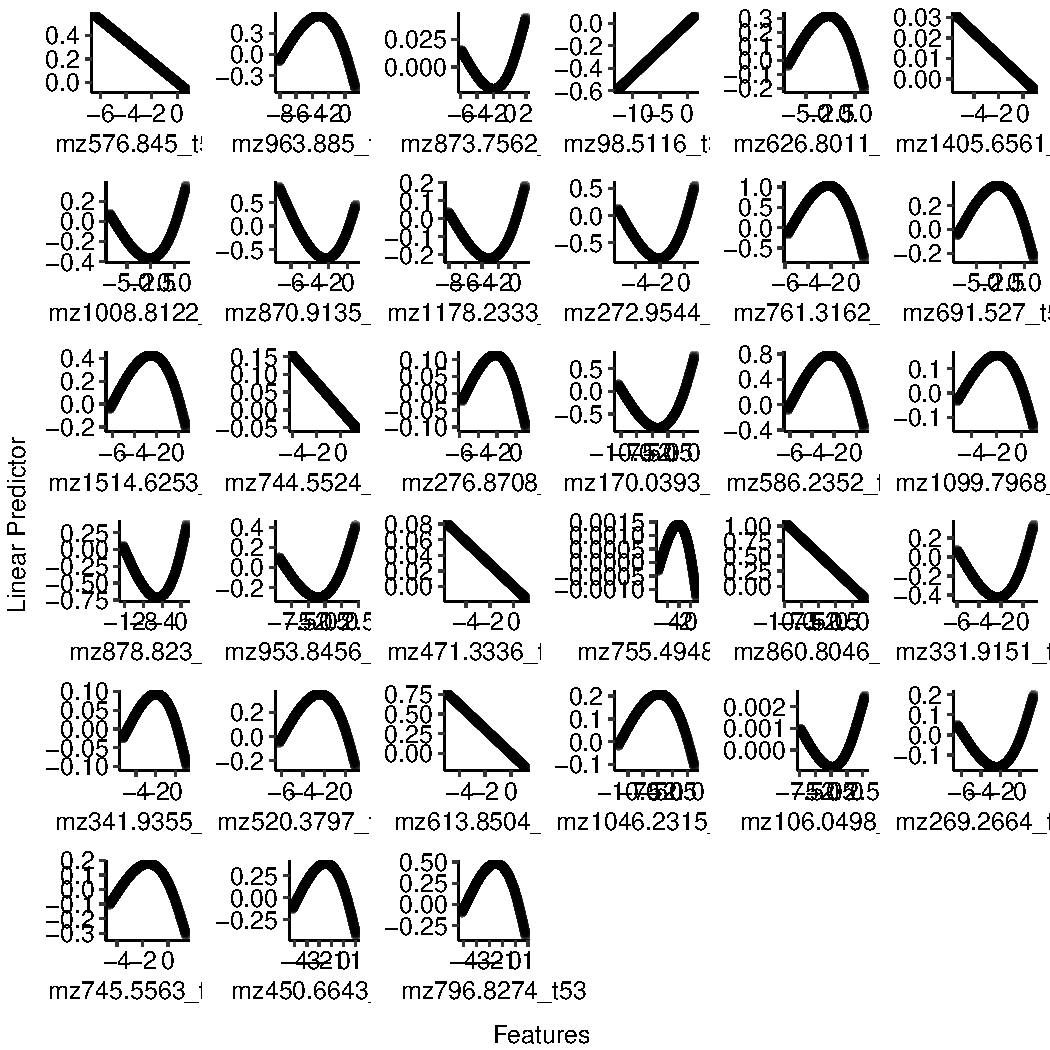
\includegraphics{Figs/ECB_plot}
\caption{Plots of the functions for the 33 metablites selected by BHAM in the Emory Cardiovascular Biobank data analysis}
\label{fig:ECB_fig}
\end{figure}



\end{document}
